\section{Results}
\subsection{Measurements of distances}
    \begin{table}[H] \small
        \centering
        \begin{tabular}{|c|c|c|c|c|}
        \hline
            & 1 & 2 & 3 & 4\\\hline
            Disk $\varnothing$ [$\e{-2}$m] $\pm$ 0.002[$\e{-2}$m] & 23.994 & 23.990 & 23.992 & 23.992\\\hline
            Hoop $\varnothing_1$ [$\e{-2}$m] $\pm$ 0.002[$\e{-2}$m] & 24.010 & 24.000 & 24.016 & 24.012\\\hline
            Hoop $\varnothing_2$ [$\e{-2}$m] $\pm$ 0.002[$\e{-2}$m] & 20.988 & 21.000 & 20.980 & 21.000\\\hline
            Cylinder A $\varnothing$ [$\e{-2}$m] $\pm$ 0.002[$\e{-2}$m] & 3.026 & 3.000 & 2.998 & 3.000\\\hline
            Cylinder B $\varnothing$ [$\e{-2}$m] $\pm$ 0.002[$\e{-2}$m] & 2.998 & 3.000 & 3.000 & 2.990\\\hline
            Cone pulley $\varnothing$ [$\e{-2}$m] $\pm$ 0.002[$\e{-2}$m] & 5.020 & 5.020 & 5.012 & 5.014\\\hline
        \end{tabular}
        \caption{Calliper measurements}\label{table_calliper}
    \end{table}
    
    \begin{table}[H] \small
        \centering
        \begin{tabular}{|c|c|c|}
        \hline
            & Inner distance & outer distance\\\hline
            Hole 1 $d$ [$\e{-2}$m] $\pm$ 0.002[$\e{-2}$m] & 3.982 & 5.028\\\hline
            Hole 2 $d$ [$\e{-2}$m] $\pm$ 0.002[$\e{-2}$m] & 4.010 & 5.022\\\hline
            Hole 3 $d$ [$\e{-2}$m] $\pm$ 0.002[$\e{-2}$m] & 7.010 & 8.028\\\hline
            Hole 4 $d$ [$\e{-2}$m] $\pm$ 0.002[$\e{-2}$m] & 6.994 & 8.026\\\hline
        \end{tabular}
        \caption{Calliper measurements for holes}\label{table_hole}
    \end{table}

    The mean values can be calculated by
    \[
        \varnothing=\frac{1}{n}\sum_{i=1}^{n}\varnothing_i.
    \]

    \textbf{For example}, for the Disk $\varnothing$ in Table \ref{table_calliper},
    \[
        \bar{\varnothing}=\frac{23.994+23.990+23.992+23.992}{4}\e{-2}=0.23992\pm0.00003m,\quad u_{\varnothing,r}=0.014\%.
    \]

    Similarly, from the raw data in Table \ref{table_calliper}, we obtain the different sets of radii.

    \begin{table}[H] \small
        \centering
        \begin{tabular}{|c|c|c|c|}
            \hline
            & mean value [m] & uncertainty [m] & relative uncertainty [\%]\\\hline
            Disk $\varnothing$ & 0.23992 & 0.00003 & 0.014\\\hline
            Hoop $\varnothing_1$ & 0.24010 & 0.00011 & 0.05\\\hline
            Hoop $\varnothing_2$ & 0.20992 & 0.00016 & 0.07\\\hline
            Cylinder A $\varnothing_A$ & 0.0301 & 0.0002 & 0.7 \\\hline
            Cylinder B $\varnothing_B$ & 0.02997 & 0.00001 & 0.3\\\hline
            Cone pulley $\varnothing_C$ & 0.05017 & 0.00007 & 0.14\\\hline
        \end{tabular}
        \caption{Average results of diameters}\label{data_diameter}
    \end{table}
    
    We know that the distances from the rotating axis to the holes are calculated by the average value of inner distance and outer distances (see Table \ref{table_hole}).

    Here's the \textbf{sample calculation} for hole 1.
    \[
        d_1=\frac{d_{1,in}+d_{1,out}}{2}=\frac{3.982+5.028}{2}\e{-2}=0.04505\pm 0.00001m,\quad u_{d_1,r}=0.03\%
    \]

    SImilarly, we obtain the data as shown in Table \ref{data_hole}.

    \begin{table}[H] \small
        \centering
        \begin{tabular}{|c|c|c|c|}
            \hline
            & mean value [m] & uncertainty [m] & relative uncertainty [\%]\\\hline
            Hole 1 $d_1$ & 0.04505 & 0.00001 & 0.03\\\hline
            Hole 2 $d_2$ & 0.04516 & 0.00001 & 0.03\\\hline
            Hole 3 $d_3$ & 0.07519 & 0.00001 & 0.02\\\hline
            Hole 4 $d_4$ & 0.07510 & 0.00001 & 0.02\\\hline
        \end{tabular}
        \caption{Average results of calliper measurements}\label{data_hole}
    \end{table}

\subsection{Measurements of mass}
    The following table shows the mass measuremnts.
    \begin{table}[H] \small
        \centering
        \begin{tabular}{|c|c|c|c|}
            \hline
            & mean value [kg] & uncertainty [kg] & relative uncertainty [\%]\\\hline
            Disk & 0.4881 & 0.0001 & 0.02\\\hline
            Hoop & 0.3998 & 0.0001 & 0.03\\\hline
            Cylinder A & 0.1660 & 0.0001 & 0.06\\\hline
            Cylinder B & 0.1660 & 0.0001 & 0.06\\\hline
            Weight & 0.0545 & 0.0001 & 0.18\\\hline
        \end{tabular}
        \caption{Mass measurements}\label{data_mass}
    \end{table}

\subsection{Measurements of the acceleration}
    In this exercise, we get the value of angular acceleration $\beta$ by $\theta$ vs. $t$ quadratic fitting. The data for curve fitting are shown in the corresponding table.
\subsubsection{Measurements for empty turntable}
    \begin{table}[H] \small
        \centering
        \begin{tabular}{|c|c|c|c|c|c|c|c|c|}
            \hline
            & \multicolumn{8}{c|}{Deceleration} \\\hline
            $\theta$ & 3.142 & 6.283 & 9.425 & 12.57 & 15.71 & 18.85 & 21.99 & 25.13\\\hline
            t[s] & 0.4748 & 0.9520 & 1.4311 & 1.9131 & 2.3975 & 2.8843 & 3.3738 & 3.8665\\\hline
            $u_t$[$\e{-3}$s] & 0.12 & 0.14 & 0.2 & 0.2 & 0.2 & 0.2 & 0.2 & 0.3\\\hline
            & \multicolumn{8}{c|}{Acceleration} \\\hline
            $\theta$ & 3.142 & 6.283 & 9.425 & 12.57 & 15.71 & 18.85 & 21.99 & 25.13\\\hline
            t[s] & 0.7761 & 1.3508 & 1.8366 & 2.2633 & 2.6480 & 3.0014 & 3.3299 & 3.6383\\\hline
            $u_t$[$\e{-3}$s] & 0.13 & 0.2 & 0.2 & 0.2 & 0.2 & 0.2 & 0.2 & 0.3\\\hline
        \end{tabular}
        \caption{Measurements for empty turntable}\label{data_1}
    \end{table}

    \begin{figure}[H]
    \centering
    \begin{minipage}{0.6\textwidth}    
        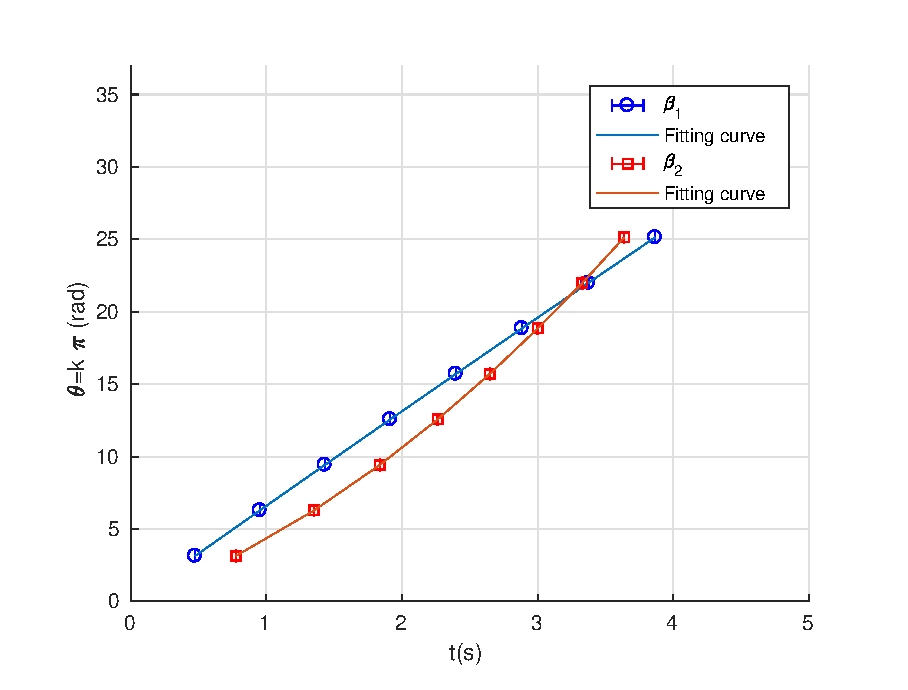
\includegraphics[width=0.9\textwidth]{images/1}
        \caption{Quadratic fitting for empty turntable}\label{fig_1}
    \end{minipage}
    ~
    \begin{minipage}{0.35\textwidth}
        \[
        \begin{split}
            \beta_1&=-0.071\pm 0.002rad/s^2,\\
            \beta_2&=1.956\pm 0.012rad/s^2.
        \end{split}
        \]
    \end{minipage}
    \end{figure}

    \begin{figure}[H]
    \centering
    \begin{minipage}{0.45\textwidth}
        \includegraphics[width=0.9\textwidth]{images/11info}
        \caption{Deceleration of empty turntable}\label{11info}
    \end{minipage}
    ~
    \begin{minipage}{0.45\textwidth}
        \includegraphics[width=0.9\textwidth]{images/12info}
        \caption{Acceleration of empty turntable}\label{12info}
    \end{minipage}
    \end{figure}

\subsubsection{Measurements for turntable with disk}
    \begin{table}[H] \small
        \centering
        \begin{tabular}{|c|c|c|c|c|c|c|c|c|}
            \hline
            & \multicolumn{8}{c|}{Deceleration} \\\hline
            $\theta$ & 3.142 & 6.283 & 9.425 & 12.57 & 15.71 & 18.85 & 21.99 & 25.13\\\hline
            t[s] & 0.6150 & 1.2334 & 1.8548 & 2.4803 & 3.1085 & 3.7404 & 4.3765 & 5.0164\\\hline
            $u_t$[$\e{-3}$s] & 0.12 & 0.15 & 0.2 & 0.2 & 0.2 & 0.2 & 0.3 & 0.3\\\hline
            & \multicolumn{8}{c|}{Acceleration} \\\hline
            $\theta$ & 3.142 & 6.283 & 9.425 & 12.57 & 15.71 & 18.85 & 21.99 & 25.13\\\hline
            t[s] & 0.9789 & 1.7085 & 2.3176 & 2.8516 & 3.3332 & 3.7747 & 4.1853 & 4.5701\\\hline
            $u_t$[$\e{-3}$s] & 0.14 & 0.2 & 0.2 & 0.2 & 0.2 & 0.3 & 0.3 & 0.3\\\hline
        \end{tabular}
        \caption{Measurements for turntable with disk}\label{data_2}
    \end{table}

    \begin{figure}[H]
    \centering
    \begin{minipage}{0.6\textwidth}    
        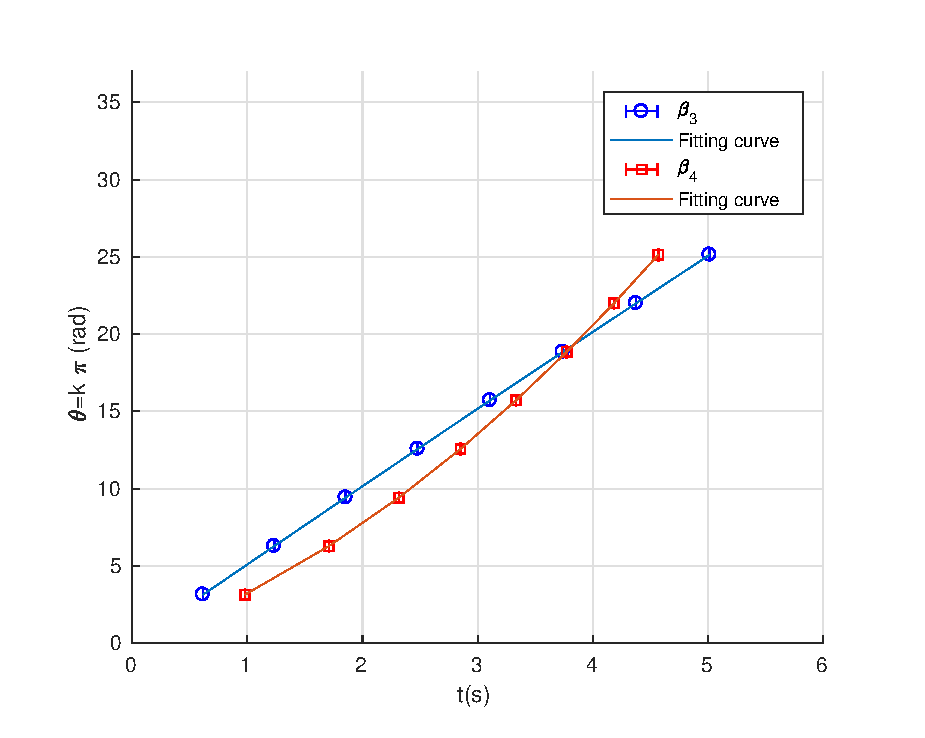
\includegraphics[width=0.9\textwidth]{images/2}
        \caption{Quadratic fitting for turntable with disk}\label{fig_2}
    \end{minipage}
    ~
    \begin{minipage}{0.35\textwidth}
        \[
        \begin{split}
            \beta_3&=-0.0452\pm 0.0013rad/s^2,\\
            \beta_4&=1.2700\pm 0.0012rad/s^2.
        \end{split}
        \]
    \end{minipage}
    \end{figure}

    \begin{figure}[H]
    \centering
    \begin{minipage}{0.45\textwidth}
        \includegraphics[width=0.9\textwidth]{images/21info}
        \caption{Deceleration of turntable with disk}\label{21info}
    \end{minipage}
    ~
    \begin{minipage}{0.45\textwidth}
        \includegraphics[width=0.9\textwidth]{images/22info}
        \caption{Acceleration of turntable with disk}\label{22info}
    \end{minipage}
    \end{figure}

\subsubsection{Measurements for turntable with hoop}
    \begin{table}[H] \small
        \centering
        \begin{tabular}{|c|c|c|c|c|c|c|c|c|}
            \hline
            & \multicolumn{8}{c|}{Deceleration} \\\hline
            $\theta$ & 3.142 & 6.283 & 9.425 & 12.57 & 15.71 & 18.85 & 21.99 & 25.13\\\hline
            t[s] & 0.5987 & 1.2010 & 1.8081 & 2.4173 & 3.0291 & 3.6429 & 4.2600 & 4.8792\\\hline
            $u_t$[$\e{-3}$s] & 0.12 & 0.15 & 0.2 & 0.2 & 0.2 & 0.2 & 0.3 & 0.3\\\hline
            & \multicolumn{8}{c|}{Acceleration} \\\hline
            $\theta$ & 3.142 & 6.283 & 9.425 & 12.57 & 15.71 & 18.85 & 21.99 & 25.13\\\hline
            t[s] & 1.1370 & 1.9548 & 2.6283 & 3.2142 & 3.7402 & 4.2213 & 4.6676 & 5.0855\\\hline
            $u_t$[$\e{-3}$s] & 0.15 & 0.2 & 0.2 & 0.2 & 0.2 & 0.3 & 0.3 & 0.3\\\hline
        \end{tabular}
        \caption{Measurements for turntable with hoop}\label{data_3}
    \end{table}

    \begin{figure}[H]
    \centering
    \begin{minipage}{0.6\textwidth}    
        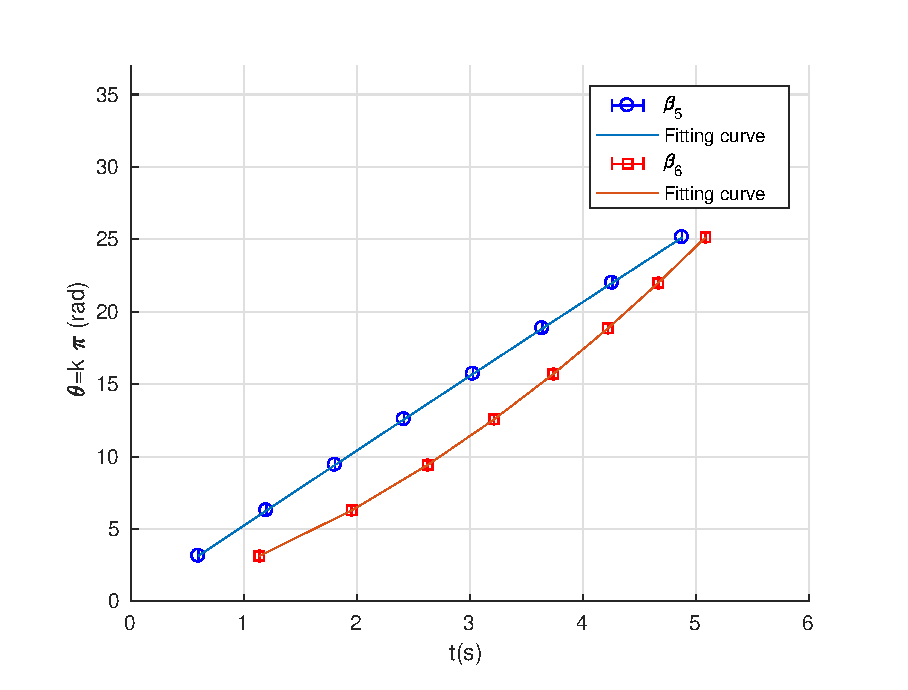
\includegraphics[width=0.85\textwidth]{images/3}
        \caption{Quadratic fitting for turntable with hoop}\label{fig_3}
    \end{minipage}
    ~
    \begin{minipage}{0.35\textwidth}
        \[
        \begin{split}
            \beta_5&=-0.036\pm 0.003rad/s^2,\\
            \beta_6&=1.1034\pm 0.0008rad/s^2.
        \end{split}
        \]
    \end{minipage}
    \end{figure}

    \begin{figure}[H]
    \centering
    \begin{minipage}{0.45\textwidth}
        \includegraphics[width=0.8\textwidth]{images/31info}
        \caption{Deceleration of turntable with hoop}\label{31info}
    \end{minipage}
    ~
    \begin{minipage}{0.45\textwidth}
        \includegraphics[width=0.8\textwidth]{images/32info}
        \caption{Acceleration of turntable with hoop}\label{32info}
    \end{minipage}
    \end{figure}

\subsubsection{Measurements for turntable with cylinder A in hole 1 and B in 2}
    \begin{table}[H] \small
        \centering
        \begin{tabular}{|c|c|c|c|c|c|c|c|c|}
            \hline
            & \multicolumn{8}{c|}{Deceleration} \\\hline
            $\theta$ & 3.142 & 6.283 & 9.425 & 12.57 & 15.71 & 18.85 & 21.99 & 25.13\\\hline
            t[s] & 0.5702 & 1.1439 & 1.7209 & 2.3022 & 2.8866 & 3.4748 & 4.0660 & 4.6609\\\hline
            $u_t$[$\e{-3}$s] & 0.12 & 0.15 & 0.2 & 0.2 & 0.2 & 0.2 & 0.3 & 0.3\\\hline
            & \multicolumn{8}{c|}{Acceleration} \\\hline
            $\theta$ & 3.142 & 6.283 & 9.425 & 12.57 & 15.71 & 18.85 & 21.99 & 25.13\\\hline
            t[s] & 0.8071 & 1.4176 & 1.9295 & 2.3788 & 2.7848 & 3.1574 & 3.5055 & 3.8331\\\hline
            $u_t$[$\e{-3}$s] & 0.13 & 0.2 & 0.2 & 0.2 & 0.2 & 0.2 & 0.2 & 0.3\\\hline
        \end{tabular}
        \caption{Measurements for turntable with cylinder A in 1 and B in 2}\label{data_4}
    \end{table}

    \begin{figure}[H]
    \centering
    \begin{minipage}{0.6\textwidth}    
        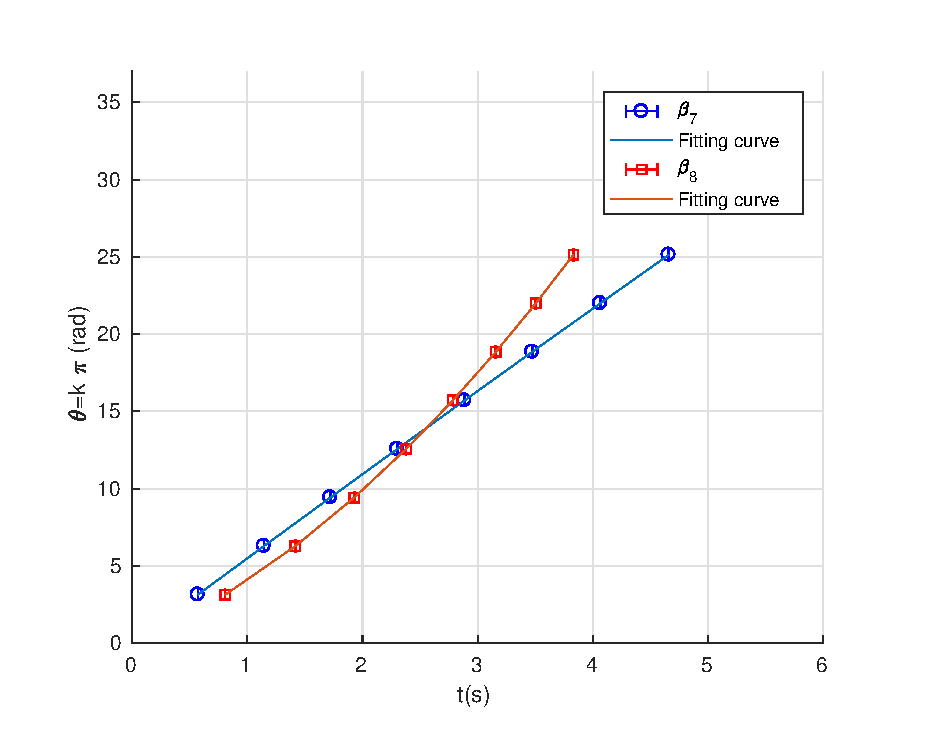
\includegraphics[width=0.8\textwidth]{images/4}
        \caption{Quadratic fitting for turntable with cylinder A in 1 and B in 2}\label{fig_4}
    \end{minipage}
    ~
    \begin{minipage}{0.35\textwidth}
        \[
        \begin{split}
            \beta_7&=-0.056\pm 0.002rad/s^2,\\
            \beta_8&=1.748\pm 0.016rad/s^2.
        \end{split}
        \]
    \end{minipage}
    \end{figure}

    \begin{figure}[H]
    \centering
    \begin{minipage}{0.45\textwidth}
        \includegraphics[width=0.8\textwidth]{images/41info}
        \caption{Deceleration of turntable with cylinder A in 1 and B in 2}\label{41info}
    \end{minipage}
    ~
    \begin{minipage}{0.45\textwidth}
        \includegraphics[width=0.8\textwidth]{images/42info}
        \caption{Acceleration of turntable with cylinder A in 1 and B in 2}\label{42info}
    \end{minipage}
    \end{figure}

\subsubsection{Measurements for turntable with cylinder A in hole 3 and B in 4}
    \begin{table}[H] \small
        \centering
        \begin{tabular}{|c|c|c|c|c|c|c|c|c|}
            \hline
            & \multicolumn{8}{c|}{Deceleration} \\\hline
            $\theta$ & 3.142 & 6.283 & 9.425 & 12.57 & 15.71 & 18.85 & 21.99 & 25.13\\\hline
            t[s] & 0.5611 & 1.1250 & 1.6916 & 2.2618 & 2.8345 & 3.4103 & 3.9888 & 4.5704\\\hline
            $u_t$[$\e{-3}$s] & 0.12 & 0.15 & 0.2 & 0.2 & 0.2 & 0.2 & 0.3 & 0.3\\\hline
            & \multicolumn{8}{c|}{Acceleration} \\\hline
            $\theta$ & 3.142 & 6.283 & 9.425 & 12.57 & 15.71 & 18.85 & 21.99 & 25.13\\\hline
            t[s] & 0.8086 & 1.4397 & 1.9758 & 2.4497 & 2.8797 & 3.2757 & 3.6453 & 3.9925\\\hline
            $u_t$[$\e{-3}$s] & 0.13 & 0.2 & 0.2 & 0.2 & 0.2 & 0.2 & 0.2 & 0.3\\\hline
        \end{tabular}
        \caption{Measurements for turntable with cylinder A in 3 and B in 4}\label{data_5}
    \end{table}

    \begin{figure}[H]
    \centering
    \begin{minipage}{0.6\textwidth}    
        \includegraphics[width=0.8\textwidth]{images/5}
        \caption{Quadratic fitting for turntable with cylinder A in 3 and B in 4}\label{fig_5}
    \end{minipage}
    ~
    \begin{minipage}{0.35\textwidth}
        \[
        \begin{split}
            &\beta_9=-0.0492\pm 0.0006rad/s^2,\\
            &\beta_{10}=1.509\pm 0.001rad/s^2.
        \end{split}
        \]
    \end{minipage}
    \end{figure}

    \begin{figure}[H]
    \centering
    \begin{minipage}{0.45\textwidth}
        \includegraphics[width=0.8\textwidth]{images/51info}
        \caption{Deceleration of turntable with cylinder A in 3 and B in 4}\label{51info}
    \end{minipage}
    ~
    \begin{minipage}{0.45\textwidth}
        \includegraphics[width=0.8\textwidth]{images/52info}
        \caption{Acceleration of turntable with cylinder A in 3 and B in 4}\label{52info}
    \end{minipage}
    \end{figure}

\subsection{Calculations for the moment of inertia}
    First, according to  United States Department of Commerce, the acceleration due to gravity in Shanghai is $9.794m/s^2$.

    Here we only have the \textbf{sample calculation} of the moment of inertia of the empty turntable.
    As stated in Eq. \ref{equ_I}, we can derive $I_1$ from the data in Table \ref{data_diameter}, \ref{data_hole} and \ref{data_mass}.
    \[
    \begin{split}
        &\beta_1=-0.071\pm 0.002 rad/s^2,\\
        &\beta_2=1.956\pm 0.012 rad/s^2,\\
        &R_{cone}=0.02509\pm0.00003 m,\\
        &m_{weight}=0.0545\pm0.0001 kg,\\
        &g=9.794m/s^2,\\
        &I_1=\frac{mR(g-R\beta_2)}{\beta_2-\beta_1}=\frac{0.0545\times0.02509\times(9.794-0.02509\times1.956)}{1.956-(-0.071)}=(0.00707\pm 0.00005)kg\cdot m^2.
    \end{split}
    \]

    Hence, $I_1=(7.07\pm 0.05) \e{-3}kg\cdot m^2, \quad u_{I_1,r}=0.7\%$.

    Simlarly, we can calculate the other moments of inertia (see Table \ref{data_I}).

    \begin{table}[H] \small
        \centering
        \begin{tabular}{|c|c|c|c|}
            \hline
            & $I$ [$\e{-3}kg\cdot m^2$] & $u_I$ [$\e{-3}kg\cdot m^2$] & $u_{I,r}$ [$\%$]\\\hline
            Empty turntable $I_1$ & 7.07 & 0.05 & 0.7\\\hline
            Turntable with disk $I_2$ & 10.90 & 0.03 & 0.3\\\hline
            Turntable with hoop $I_3$ & 12.51 & 0.05 & 0.4\\\hline
            A in 1 \& B in 2 $I_4$ & 7.88 & 0.08 & 1.0\\\hline
            A in 3 \& B in 4 $I_5$ & 9.14 & 0.02 & 0.2\\\hline
        \end{tabular}
        \caption{Results for the moments of inertia (combined)}\label{data_I}
    \end{table}

    Finally, due to the additivity of the moment of inertia, we calculate the difference.

    \textbf{For example}, for the turntable with disk, we know that
    \[
        I_{disk}=I_2-I_1=(3.83\pm 0.06)\e{-3}kg\cdot m^2.
    \]

    \begin{table}[H] \small
        \centering
        \begin{tabular}{|c|c|c|c|}
            \hline
            & $I$ [$\e{-3}kg\cdot m^2$] & $u_I$ [$\e{-3}kg\cdot m^2$] & $u_{I,r}$ [$\%$]\\\hline
            $I_{empty}$ & 7.07 & 0.05 & 0.7\\\hline
            $I_{disk}$ & 3.83 & 0.06 & 1.5\\\hline
            $I_{hoop}$ & 5.44 & 0.07 & 1.2\\\hline
            $I_{1,2}$ & 0.81 & 0.09 & 11\\\hline
            $I_{3,4}$ & 2.07 & 0.05 & 3\\\hline
        \end{tabular}
        \caption{Results for the moments of inertia}\label{data_i}
    \end{table}

\subsection{Calculations for theoretical value of moment of inertia}
    Since it's the theoretical value of moment of inertia, then we just consider it as the precise value without uncertainty. The following table shows the conslusion of theoretical values and the specific calculations are presented respectively.
    \begin{table}[H] \small
        \centering
        \begin{tabular}{|c|c|}
            \hline
            & $I_t$ [$\e{-3}kg\cdot m^2$]\\\hline
            $I_{disk}$ & 3.51\\\hline
            $I_{hoop}$ & 5.08\\\hline
            $I_{1,2}$ & 0.72\\\hline
            $I_{3,4}$ & 1.91\\\hline
        \end{tabular}
        \caption{Results for theoretical moments of inertia}\label{data_i}
    \end{table}
\subsubsection{Theoretical Moment inertia of disk}
    Recall the measurements for the disk (see Table \ref{data_diameter} and \ref{data_mass}).
    \[
    \begin{split}
        &m_{disk}=0.4881kg.\\
        &R_{disk}=0.23992/2=0.11996m.\\
    \end{split}
    \]

    According to the formula of moment of inertia, we obtain that
    \[
        I_{disk}=\frac{1}{2}m_{disk}R_{disk}^2=\frac{1}{2}\times 0.4881\times 0.11996^2=3.51\e{-3}kg\cdot m^2.
    \]

\subsubsection{Theoretical Moment inertia of hoop}
    Recall the measurements for the hoop (see Table \ref{data_diameter} and \ref{data_mass}).
    \[
    \begin{split}
        &m_{hoop}=0.3998kg.\\
        &R_{hoop,in}=0.20992/2=0.10496m.\\
        &R_{hoop,out}=0.24010/2=0.12005m.\\               
    \end{split}
    \]

    According to the formula of moment of inertia, we obtain that
    \[
    \begin{split}
        I_{hoop}&=\frac{1}{2}m_{hoop}(R_{hoop,in}^2+R_{hoop,out}^2)=\frac{1}{2}\times 0.3998\times (0.10496^2+0.12005^2)\\
        &=5.08\e{-3}kg\cdot m^2.
    \end{split}
    \]

\subsubsection{Theoretical Moment inertia of cylinder condition}
    Recall the measurements for the cylinder A in hole 1 and B in 2 (see Table \ref{data_diameter} and \ref{data_mass}).
    \[
    \begin{split}
        &m_{A}=0.1660kg,\\
        &m_{B}=0.1660kg,\\
        &R_{A}=0.0301/2=0.01505m,\\
        &R_{B}=0.02997/2=0.014985m,\\
        &d_1=0.04505m,\\
        &d_2=0.04516m.
    \end{split}
    \]

    According to the formula of moment of inertia, we obtain that
    \[
    \begin{split}
        I_{A}&=\frac{1}{2}m_{A}R_{A}^2=\frac{1}{2}\times 0.1660\times 0.01505^2=1.88\e{-5}kg\cdot m^2.\\
        I_{B}&=1.86\e{-5}kg\cdot m^2.\\
    \end{split}
    \]

    Accoring to the parallel axis theorem, we know that
    \[
    \begin{split}
        I_{1,2}&=I_A+m_A d_1^2+I_B+m_B d_2^2\\
        &=1.88\e{-5}+0.1660\cdot 0.04505^2+1.86\e{-5}+0.1660\cdot 0.04516^2=0.72\e{-3}kg\cdot m^2.
    \end{split}
    \]

    Similarly, we can derive $I_{3,4}$,
    \[
        I_{3,4}=1.91\e{-3}kg\cdot m^2.
    \]